\begin{figure}[tb]
\centering
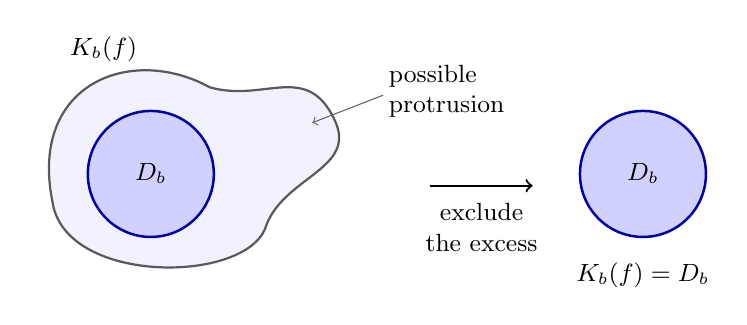
\begin{tikzpicture}[x=1cm,y=1cm,font=\small]
 \filldraw[fill=blue!5,draw=black!65,line width=.8pt]
 (-1.6,-.2) .. controls (-1.9,1.3) and (-.6,1.8) .. (.4,1.25)
 .. controls (1.1,1.05) and (1.65,1.6) .. (2,.8)
 .. controls (2.25,.2) and (1.3,.1) .. (1.1,-.55)
 .. controls (.8,-1.25) and (-1.45,-1.25) .. (-1.6,-.2);
 \filldraw[fill=blue!18,draw=blue!65!black,line width=.9pt]
 (-.35,.15) circle (.8);
 \node at (-.35,.15) {$D_b$};
 \node[above] at (-.95,1.45) {$K_b(f)$};
 \draw[->,black!60] (2.6,1.15)--(1.7,.8);
 \node[right,align=left] at (2.55,1.2) {possible\\protrusion};
 \draw[->,line width=.8pt] (3.2,0)--(4.5,0);
 \node[below,align=center] at (3.85,-.1) {exclude\\the excess};
 \filldraw[fill=blue!18,draw=blue!65!black,line width=.9pt]
 (5.9,.15) circle (.8);
 \node at (5.9,.15) {$D_b$};
 \node[below] at (5.9,-.85) {$K_b(f)=D_b$};
\end{tikzpicture}
\caption{A distinguished disk may initially be only part of a limiting
complementary component. The marked-component argument excludes every
such protrusion. This is a schematic picture; no boundary regularity of
$K_b(f)$ is assumed.}
\label{fig:protrusion}
\end{figure}
